%\let\uppercase\relax
%\addtolength{\paperheight}{+10000pt}
%\addtolength{\paperwidth}{+100pt}

\vspace{24pt}

\chapter[\textbf{Running Multiple Instances of a Program}]{Running Multiple Instances of a Program}
  %\addcontentsline{toc}{chapter}{Glassary}
In scientific computing, an often-occurring bottleneck is the collection of data.  Whether it be the result of running one simulation, two simulations, or many simulations, a particular research problem can easily take days of computer time to run.  Therefore, a major goal of many  programming languages and software packages is the optimization of computer resources.

The two branches of modern scientific computing concerned with this optimization of computer resources are: high-performance computing (HPC) and high-throughput computing (HTC).  The main distinctions between the two is that HPC focuses on decreasing the runtime of a single simulation, while HTC focuses on increasing the throughput of many simulations.  In terms of timescales, HPC maximizes the floating operations per second (FLOPS), whereas HTC maximizes the total number of operations done per month or even per year.

In the case of running multiple instances of a program, as is needed for timing shocks, HTC is usually the primary mode of optimization.  Practically, this is done when a single instance of a program runs relatively quickly and would, therefore, not receive dramatic increases in throughput from HPC.  As this number of program instances approaches the hundreds and the thousands, though, manual modification and simulation becomes intractable.  Methods for automation then become needed; this is why AHAB -- or Automated HTC Achieved with Batch Processing -- was created.

  \section{Conducting Parameter Sweeps with AHAB}
  %\addcontentsline{toc}{section}{Glossary}

AHAB -- or Automated High-throughput computing Achieved with Batch processing -- is a program used to conduct parameter sweeps over other programs' variables. This is done by using a syntax that allows new, independent variables to be created.  This is useful in a practical sense for optimization studies and for debugging.  For Shock Ignition, AHAB was used to time the three pedestal pulses, see Section\,\ref{sec:pedestal}.

A parameter sweep, or a Cartesian product, is a method for creating every combination of a set of variables and their corresponding set of value lists.  Fig.\,\ref{fig:parameterSweep} shows one example of a parameter sweep done over a coin and a six-sided die that produces twelve combinations.  Another example is the fifty-two combination parameter sweep a deck of playing cards does over its four suits and thirteen ranks.

In the two parameter sweep examples given so far, only scalar variables were used.  For Bucky, a one-dimensional code, the ability to sweep over one-dimensional vectors is also extremely important.  This was the motivation behind developing a syntax that allows new, independent variables to be created.

\sidecaptionvpos{figure}{c}
\begin{SCfigure}[][h!]	
	\centering
	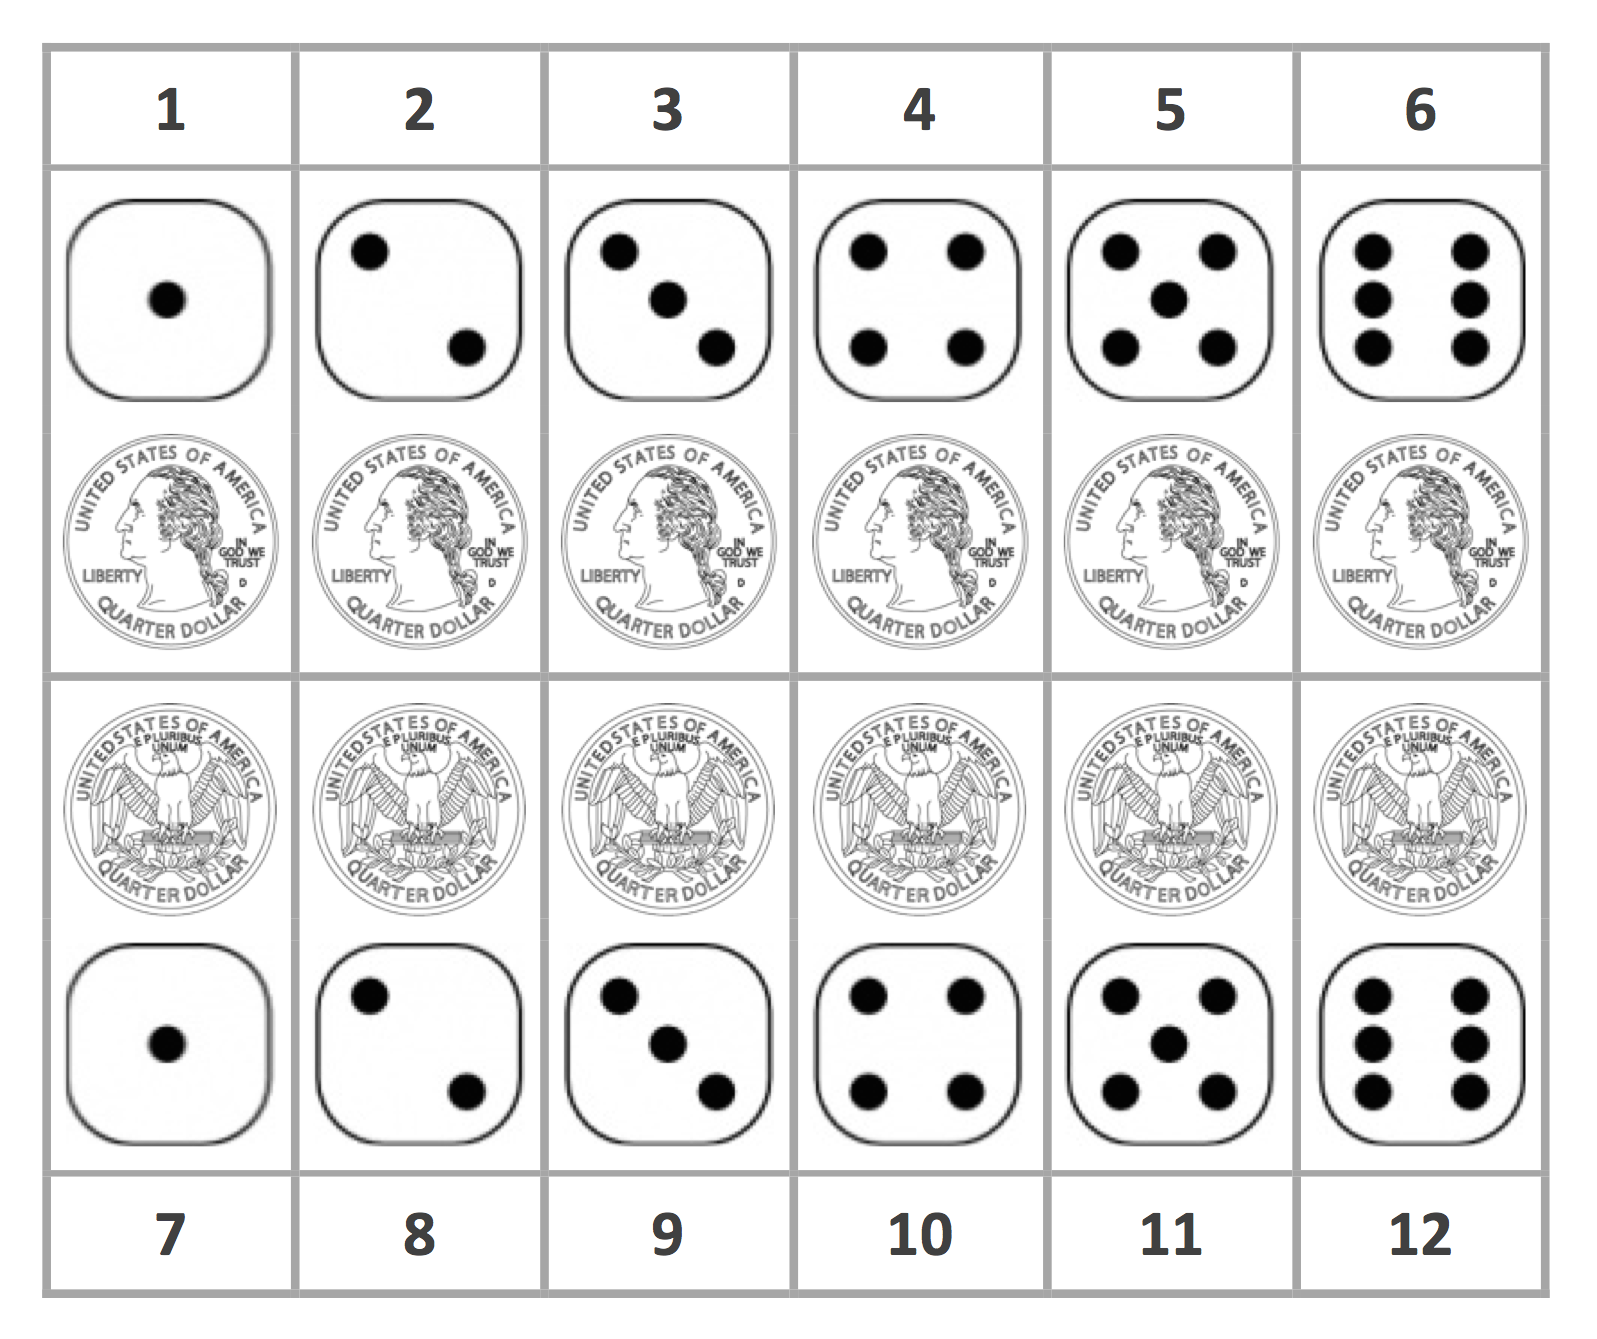
\includegraphics[width=.75\textwidth]{graphics/parameterSweep.png}
	\caption[A Scalar Parameter Sweep]{ \\ A Parameter Sweep \\ \captiontitlefinal{\textmd{over a six-sided die and a quarter.  \\ \\ Notice here that both the six-sided die and the quarter exist in a class of objects that have N distinct faces: A quarter has two faces and a six-sided die has six.  With AHAB, both these objects could be abstracted to have any multiple number of faces.} } }
	\label{fig:parameterSweep}
\end{SCfigure}
\sidecaptionvpos{figure}{b}

To get AHAB sweeping over one-dimensional vectors, though, a syntax and a construct were needed.  The syntax was needed to assist with input file parsing (see Fig.\,\ref{fig:ahabInput}), while the construct was needed to set up the logic of the sweeps (see Fig.\,\ref{fig:ahabInsert}).

AHAB's construct is how it treats variables.  This includes the distinction between: scalar and vector, completely new and old, independent values and values in sets.  Fig.\,\ref{fig:ahabInsert} shows a basic example of how this construct would handle three different variables.

The difference between the three variables in Fig.\,\ref{fig:ahabInsert} is their form of insertion.  This notion of insertion characterizes how combinations are created for the parameter sweep.  Variable (a) and variable (b) use the simpler insertions, whereas variable (c) uses a combination of the two.  

Notice in Fig.\,\ref{fig:ahabInsert} that variable (a) does not create a new combination, this is why dual insertion works: at each step of its vertical insertion process, a horizontal insertion takes place. Although the figure suggests that vertical insertion can only exist in one dimension, it can in fact take up any number of them.

\sidecaptionvpos{figure}{c}
\begin{SCfigure}[][h!]	
	\centering
	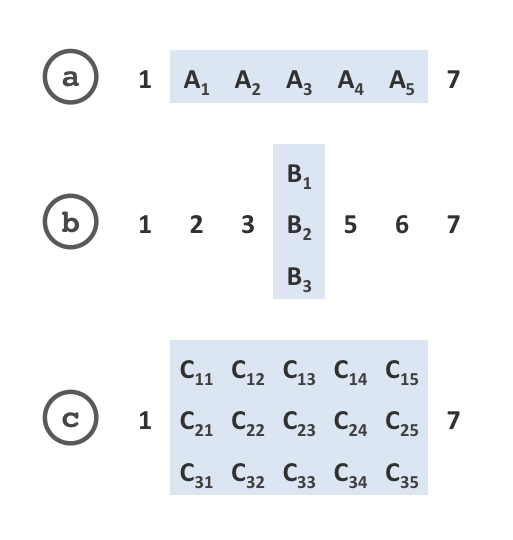
\includegraphics[width=.7\textwidth]{graphics/ahabInsert.png}
	\caption[A Vector Parameter Sweep]{ \\ A Parameter Sweep \\ \captiontitlefinal{\textmd{over three 1-D vectors. \\ \\ \textbf{(a)} uses horizontal insertion to construct large vectors. \\ \\ \textbf{(b)} uses vertical insertion to create a new vector for each value of B. \\ \\ \textbf{(c)} uses dual insertion to construct many large vectors.  It does this by using new, independent variables to combine both horizontal insertion and vertical insertion.  } } }
	\label{fig:ahabInsert}
\end{SCfigure}
\sidecaptionvpos{figure}{b}

To accomplish dual insertion, a method to add new, independent variables was needed.  In AHAB, these variables are called constants.  Fig.\,\ref{fig:ahabInput} shows how two constants, \textbf{t0} and \textbf{tDeltaFrac}, can be used to set up several vectors: \textit{tn2c}, \textit{te2c}, and \textit{tr2c}.

Fig.\,\ref{fig:ahabInput} also demonstrates several forms of syntax used by AHAB.  The \textbf{"@"} is used for constants.  The \textbf{"!"} and \textbf{"\#"} are used for comments.  The \textbf{";"} and \textbf{"|"} are used for incrementation.  And the brackets are used to distinguish vectors.  This only scratches the surface of AHAB's syntax, but gives a good overview of its use of special characters.

Lastly, notice that there are several ways to set values.  in Fig.\,\ref{fig:ahabInput}, semicolons are used to do logarithmic spacing between two values; while pipes are used to linearly increment values starting at a certain number.  This allows large lists to be constructed concisely.

\sidecaptionvpos{figure}{c}
\begin{SCfigure}[][h!]	
	\centering
	\fbox{
		\parbox{.67\linewidth}{ \texttt{
\\
\# -------------------------------------- \\
\# \ \ init ; final ; numVals  //   ( log ) \\
\# -------------------------------------- \\
\\
\phantom \ \ @t0  \ \ \ \ \ \ \ \  ! initial temperature \\
\\
\phantom \ \ \ \ \ \ \	1e-2   ;   1e+2   ;   3 \\
\\
\phantom \ \ @tDeltaFrac           !  temperature fraction \\
\\
\phantom \ \ \ \ \ \ \	100 \   ;   1000   ;   2 \\
\\
\# ---------------------------- \\
\#  \ init | increment | numVals  \\
\# ---------------------------- \\
\\
\phantom \ \ tn2c =  [ ( @t0 | @"t0/tdeltafrac" | 250 ) ] \\
\phantom \ \ te2c  \ \  [ ( @t0 | @"t0/tdeltafrac" | 250 ) ] \\
\phantom \ \ tr2c =  [ ( @t0 | @"t0/tdeltafrac" | 250 ) ] \\

		} \vspace{.15in} } 
	}
\caption[An AHAB Input File]{ \\ An Example \\ AHAB Input File \\ \captiontitlefinal{\textmd{originally used for debugging. \\ \\ Its goal was to test a new physics model for Bucky on a wide range of temperatures. This was done by setting the initial temperatures for the 250 zones' ions, electrons, and radiation. \\ \\ Here, each temperature vector would start at a value of t0 and be increased two hundred and fifty times in equal increments of t0 divided by the current value of tDeltaFrac. } } }
	\label{fig:ahabInput}
\end{SCfigure}
\sidecaptionvpos{figure}{b}







\section{Utilizing HTCondor and a Network of Computers}

As the number of combinations from parameter sweeps increases, it becomes unwieldy to run every simulation on one computer.  To remedy this problem, AHAB uses HTCondor as a method to distribute its simulations across a network of computers.  This required Bucky's start mode capabilities to be redesigned, see Appendix\,\ref{app:restart}.


\sidecaptionvpos{figure}{b}
\begin{SCfigure}[][h!]	
	\centering
	
\includegraphics[width=.72\textwidth]{graphics/HTCondor.png}
	\caption[HTCondor]{ HTCondor \\ \captiontitlefinal{\textmd{allows users to utilize a computer network's underutilized cycles.  } } }
	\label{fig:HTCondor}
\end{SCfigure}
\sidecaptionvpos{figure}{b}

HTCondor is an open-source project used for high-throughput computing (HTC).  It was created in 1984 by Miron Livny at the University of Wisconsin - Madison and was heavily developed by Michael Litzkow.  Currently, HTCondor is used at NASA, CERN, and several dozen universities \citep{htc}.   







HTCondor works by matching a user with a specific computer on their network.  Due to HTCondor's persistent motto to "leave the owner in control, regardless of the cost," matched computers are ones qualified as low-activity \citep{htc}.  On a network integrated into a computer lab, this practically means that simulations run fastest at night.

When simulations are run during peak-use times, they will frequently be lifted off busy computers and restarted on unused ones.  To allow this process to behave robustly, HTCondor offers the "Standard Universe."  This mode does, however, require a program to be compiled directly with HTCondor.  When it is difficult or impossible to do so, the "Vanilla Universe" must be used.  

Bucky uses the "Vanilla Universe" because its CMake file does not easily allow for the HTCondor compiler to be used.  In terms of development, this means that Bucky must be able to handle automatic restarts without the loss of data.  This was why the Automatic Mode was created in Bucky, see Appendix\,\ref{app:restart}.

